\section*{Exercise 3}

\subsection*{rep-10}
\begin{figure}[H]
\center
	\begin{subfigure}[b]{0.49\textwidth}
	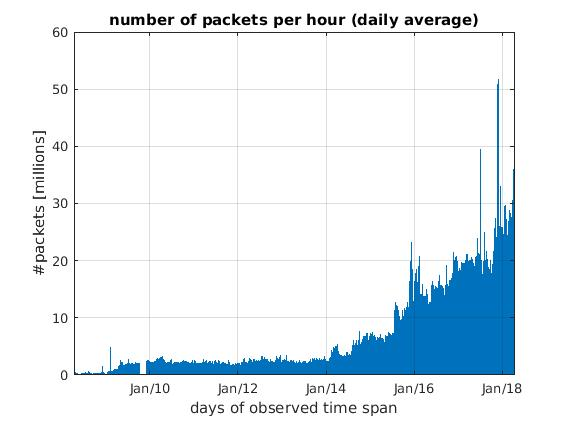
\includegraphics[width=\textwidth]{./chapters/plots/rep10_1.jpg}\\
	\end{subfigure}
	~
	\begin{subfigure}[b]{0.49\textwidth}
	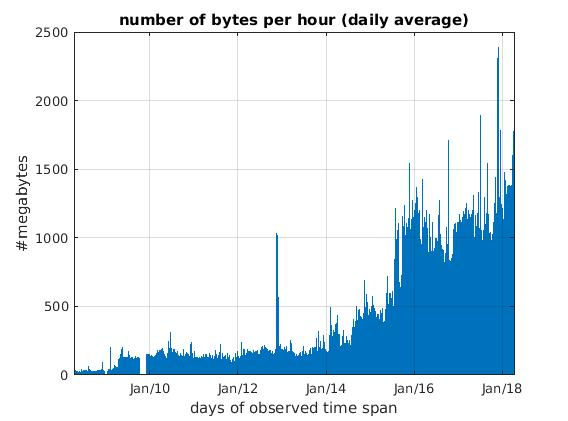
\includegraphics[width=\textwidth]{./chapters/plots/rep10_2.jpg}\\
	\end{subfigure}
	\caption{Results of rep10-1 (left) and rep10-2 (right)}
\end{figure}

\begin{figure}[H]
\center
	\begin{subfigure}[b]{0.49\textwidth}
	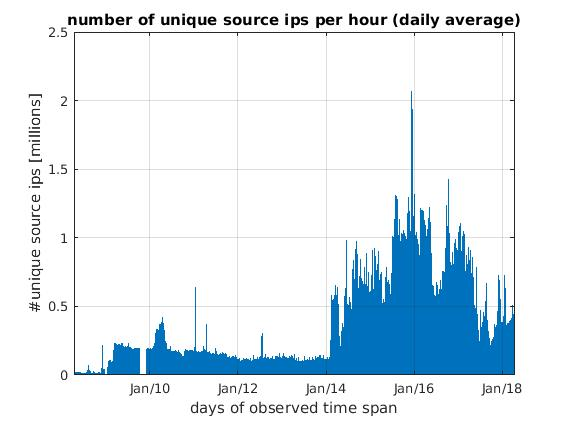
\includegraphics[width=\textwidth]{./chapters/plots/rep10_3.jpg}\\
	\end{subfigure}
	~
	\begin{subfigure}[b]{0.49\textwidth}
	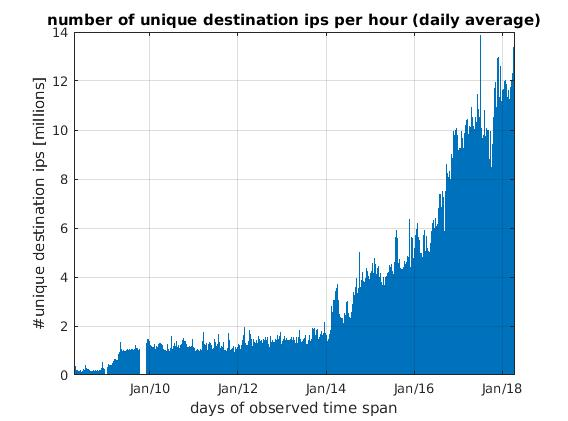
\includegraphics[width=\textwidth]{./chapters/plots/rep10_4.jpg}\\
	\end{subfigure}

	\caption{Results of rep10-3 (left) and rep10-4 (right)}
\end{figure}

\begin{figure}[H]
\center
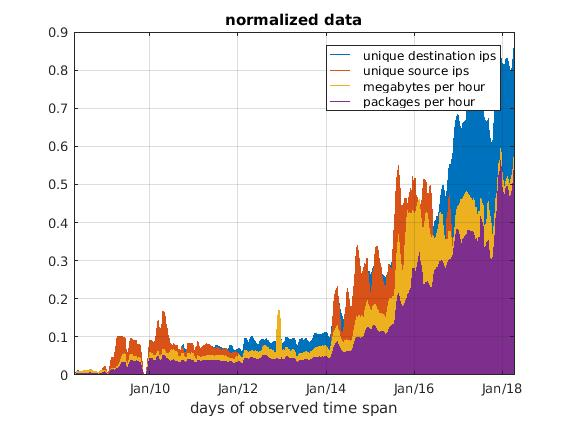
\includegraphics[width=.5\textwidth]{./chapters/plots/rep10_5.jpg}\\
\caption{Results of rep10-5}
\end{figure}





\subsection*{rep-11}
For this task, the correlation matrix was calculated by executing the matlab code of listing~\ref{lst:correlation}.

\lstinputlisting[label={lst:correlation},
				caption=Matlab code for calculating the minimal correlation]
				{./chapters/matlab/team16_ex3_rep11.m}

The correlation matrix presented in figure~\ref{fig:correlation} shows us, that the \text{\#unique source IP addresses per hour} show the lowest correlation values, especially with the \textit{\#unique destination IP addresses per hour}. It is noticeable, that there is a drop after Jan/16 for the unique IP sources. This drop does slightly correlate with the other features. This may be a result of a botnet stopping connecting to the darkspace. The botnet may tried to do a horizontal scan.

\begin{figure}[H]
\center
$
\begin{bmatrix}
1.000 &  0.965 &  0.720 &  0.934 \\
0.965 &  1.000 &  0.610 &  0.973 \\
0.720 &  0.610 &  1.000 &  0.589 \\
0.934 &  0.973 &  0.589 &  1.000
\end{bmatrix}
$
\caption{ Correlation matrix of the dataset containing the values for all 4 features }
\label{fig:correlation}
\end{figure}

\subsection*{rep-12}
In order to find out, if there are more sources sending data to the darkspace, than addresses receiving data from it, the ratio between the unique source and destination IPs is calculated, as shown in listing~\ref{lst:ratio_source_destination_ip}.

\lstinputlisting[label={lst:ratio_source_destination_ip},
				caption=Matlab code for calculating the ratio between the average unique source addresses and the average unique destination addresses per hour]
				{./chapters/matlab/team16_ex3_rep12_less.m}


The ratio between source and destination IPs is 9.31. This means, that there are approximately 10 times more addresses receiving data from the darkspace. This result was expected, as \textit{rep-11} already showed, that there may be a horizontal scan going on.

\subsection*{rep-13}
To find the peak of the '\#uIPs/hour (daily avg.)', the first column was converted to datenum format before retrieving the maximum value of the '\#uIPs/hour (daily avg.)' column. The \textit{max} function retrieves the maximum value and it's index. \\
The peak occurred on the \textbf{15th of December 2015}. As the neighbour values (14th and 16th of December) are significantly smaller, the peak lasted only for one day.

\subsection*{rep-14}
Table~\ref{tab:stat_jun2017_gen} shows the statistical values for the file \textit{Jun2017\_gen.csv} and table~\ref{tab:stat_jun2017_global} shows statistical values for the same time period, but the data was extracted from the \textit{global\_last10years.csv}. 

\begin{table}[H]
\center
\begin{tabular}{lrrrr}
\toprule
feature & total sum & mean & median & standard deviation \\
\midrule
\#pkts/hour & 6 922.229  &   9.695  &    9.937  &   1.443 \\
\#bytes/hour & 207.103  &   0.290   &   0.241  &   0.098 \\
\#uIPs/hour  & 13 157.867  &  18.428  &   18.511 &    4.329 \\
\#uIPd/hour  & 719 606.146 &  1 007.852 &   993.364 &  237.632 \\
\bottomrule
\end{tabular}
\caption{Statistics of June 2017 from Jun2017\_gen.csv (in millions)}
\label{tab:stat_jun2017_gen}
\end{table}

\begin{table}[H]
\center
\begin{tabular}{lrrrr}
\toprule
feature & total sum & mean & median & standard deviation \\
\midrule
\#pkts/hour  &    291.275  &      9.709  &      9.996   &    1.169 \\
\#bytes/hour &      8.700  &      0.290  &      0.254   &    0.076 \\
\#uIPs/hour  & 30 268.997  &  1 008.967  &  1 008.526   &  101.158\\
\#uIPd/hour  &    553.823  &     18.461  &     19.124   &    3.080 \\
\bottomrule
\end{tabular}
\caption{Statistics of June 2017 from global\_last10years.csv (in millions)}
\label{tab:stat_jun2017_global}
\end{table}

\subsection*{rep-15}
Comparing table~\ref{tab:stat_jun2017_gen} and table~\ref{tab:stat_jun2017_global} leads to the conclusion, that some values do coincide, but not all. Especially int the \textit{total sum} column are big differences. The problem is, that in the table~\ref{tab:stat_jun2017_gen} the averages for every hour are summed up and compared to the averaged value of the second table, therefore it is not surprising, that the \textit{total sum} values of~table \ref{tab:stat_jun2017_global} are significantly smaller.
There are also differences, when it comes to '\#uIPs/hour' and '\#uIPd/hour'. The problem here is, that in the table~\ref{tab:stat_jun2017_gen}, the same IP occurring every hour of the same day, is counted as a unique IP, where as in table \ref{tab:stat_jun2017_global} this IP address would be counted for the whole day as \textbf{one} unique IP address.
Mean, median and standard deviation values for '\#pkts/hour' and '\#bytes/hour' are not sensitive to those problems, therefore they do coincide in both tables.

\subsection*{rep-16}
The protocols found in the 'Jun2017\_proto.csv' file are listed in table~\ref{tab:proto}. The protocol name for each number can be found here: \url{https://www.iana.org/assignments/protocol-numbers/protocol-numbers.xhtml}

\begin{table}[H]
\center
\begin{tabular}{lrp{5cm}}
\toprule
	Protocol No. & Name & Description \\
\midrule
	1 & ICMP & The Internet Control Message Protocol is used for reporting status informations or error messages in IP, TCP and UDP protocols. Especially Gateways and Hosts use this Protocol for reporting problems. \tablefootnote{\url{https://www.itwissen.info/ICMP-Internet-control-message-protocol-ICMP-Protokoll.html}}\\
	6 & TCP & The Transmission Control Protocol is one of the main protocols of the internet. It provides reliable, ordered and error-checked delivery of bytes. \tablefootnote{\url{https://en.wikipedia.org/wiki/Transmission_Control_Protocol}} \\
	17 & UDP & The User Datagram Protocol is one of the core members of the internet. The big difference to TCP is, that it is connection less, which means, that data can be send, without the need to set up communication channels or data paths. \tablefootnote{\url{https://en.wikipedia.org/wiki/User_Datagram_Protocol
}}\\
\bottomrule
\end{tabular}
\caption{ The protocols been found in 'Jun2017\_proto.csv' }
\label{tab:proto}
\end{table}

\subsection*{rep-17}
\subsubsection*{Statistics}
\begin{table}[H]
\center
\begin{tabular}{lrrr}
\toprule
protocol & mean (in millions) & median (in millions) & standard deviations \\
\midrule
ICMP &   16.525  &  16.325  &  25.355 \% \\
TCP &     1.747  &   1.674  &  39.693 \% \\
UDP &     0.184  &   0.149  &  83.086 \% \\
others &  0.019  &   0.019  &  33.273 \% \\
\bottomrule
\end{tabular}
\caption{ Packets statistics }
\label{tab:proto-stats-packets}
\end{table}

\begin{table}[H]
\center
\begin{tabular}{lrrr}
\toprule
protocol & mean (in millions) & median (in millions) & standard deviations \\
\midrule
ICMP &    0.223 & 19.105 &   29.895 \% \\
TCP &     0.077 &  0.050 &   59.264 \% \\
UDP &     0.012 &  0.004 &  276.280 \% \\
others & -0.021 & -0.005 & -123.326 \% \\
\bottomrule
\end{tabular}
\caption{ uIPs statistics }
\label{tab:proto-stats-uIPs}
\end{table}

\begin{table}[H]
\center
\begin{tabular}{lrrr}
\toprule
protocol & mean (in millions) & median (in millions) & standard deviations \\
\midrule
ICMP &    9.253 &  9.448 &  14.728 \%  \\
TCP &     1.055 &  1.049 &  35.417 \%  \\
UDP &     0.155 &  0.120 &  92.408 \%  \\
others & -0.744 & -0.724 & -40.126 \%  \\
\bottomrule
\end{tabular}
\caption{ uIPd statistics }
\label{tab:proto-stats-uIPd}
\end{table}

\subsubsection*{Boxplots}
\begin{figure}[H]
\center
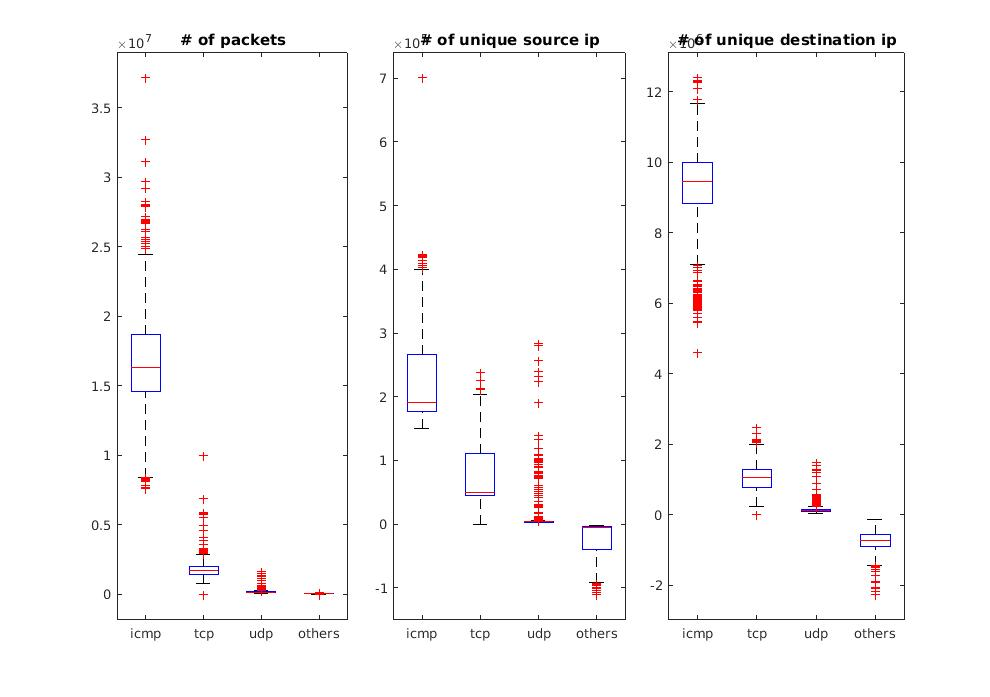
\includegraphics[width=.7\textwidth]{./chapters/plots/rep17.jpg}\\
\caption{Boxplots of \textit{rep-17}}
\end{figure}


\subsection*{rep-18}
Yes, there are negative values for '\#uIPs/hour' and '\#uIPd/hour'. In case one and the same host uses all three protocols in the same hour, this ip address is going to be counted three times (for each protocol). But in the 'Jun2017\_gen.csv' file it will be counted only one time. In this case we would end up with a 'others' value in the '\#uIPs/hour' table of $1 - (1+1+1) = -2$. The same applies to the '\#uIPd/hour'. The 'packets' values are not affected, as every packet refers to \textbf{exactly one} protocol.
% \section*{rep-19} OPTIONAL
% \section*{rep-20} OPTIONAL

\subsection*{rep-21}
\subsubsection*{a)}
\begin{figure}[H]
\center
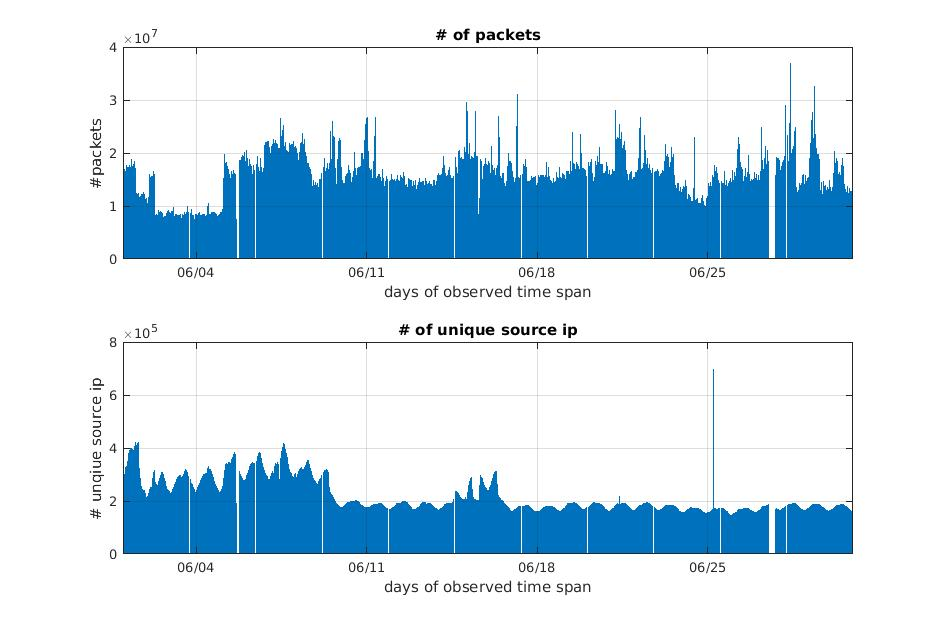
\includegraphics[width=.7\textwidth]{./chapters/plots/rep21a.jpg}\\
\caption{ Time series of \# of packets and \# of usIP }
\end{figure}

\subsubsection*{b)}
\begin{figure}[H]
\center
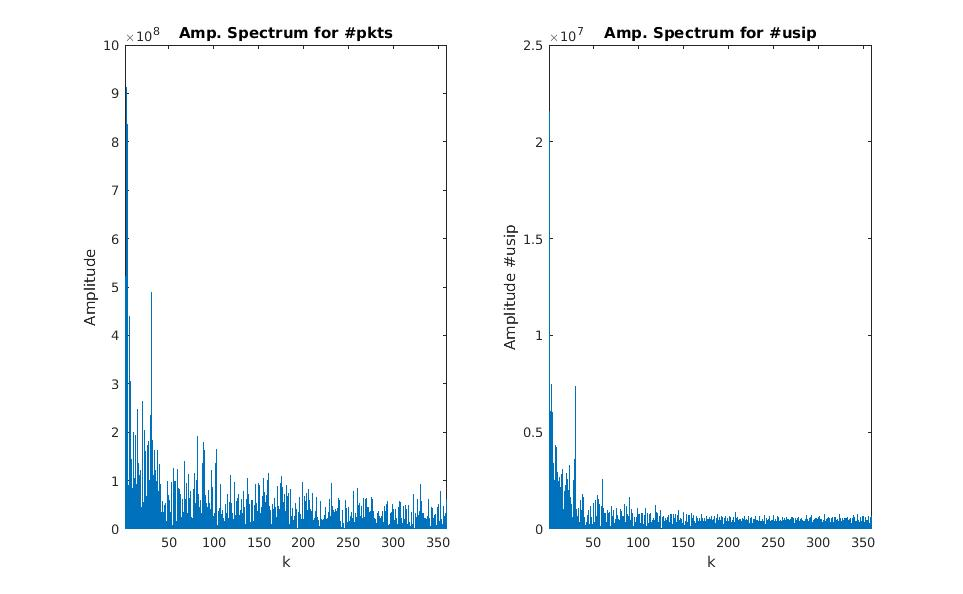
\includegraphics[width=.7\textwidth]{./chapters/plots/rep21b.jpg}\\
\caption{ FFT of \# of packets and \# of usIP  }
\end{figure}

\subsubsection*{c)}
The \textit{\#pkts/hour} and the \textit{\#uIPs/hour} show periodicity.\\

\textit{\#pkts/hour} has a periodicity with an amplitude of $9.1372 * 10^8$ at k=3. This complies with a period of 240 hours. \\

For \textit{\#uIPs/hour} there is a periodicity for k = 1. At this point the amplitude is $21.5964 * 10^6$. k = 1 corresponds to a period of 720 hours. \\

In addition, both signals have a peak at k=30, which corresponds to a period of 24 hours.

\subsection*{rep-22}
\begin{figure}[H]
\center
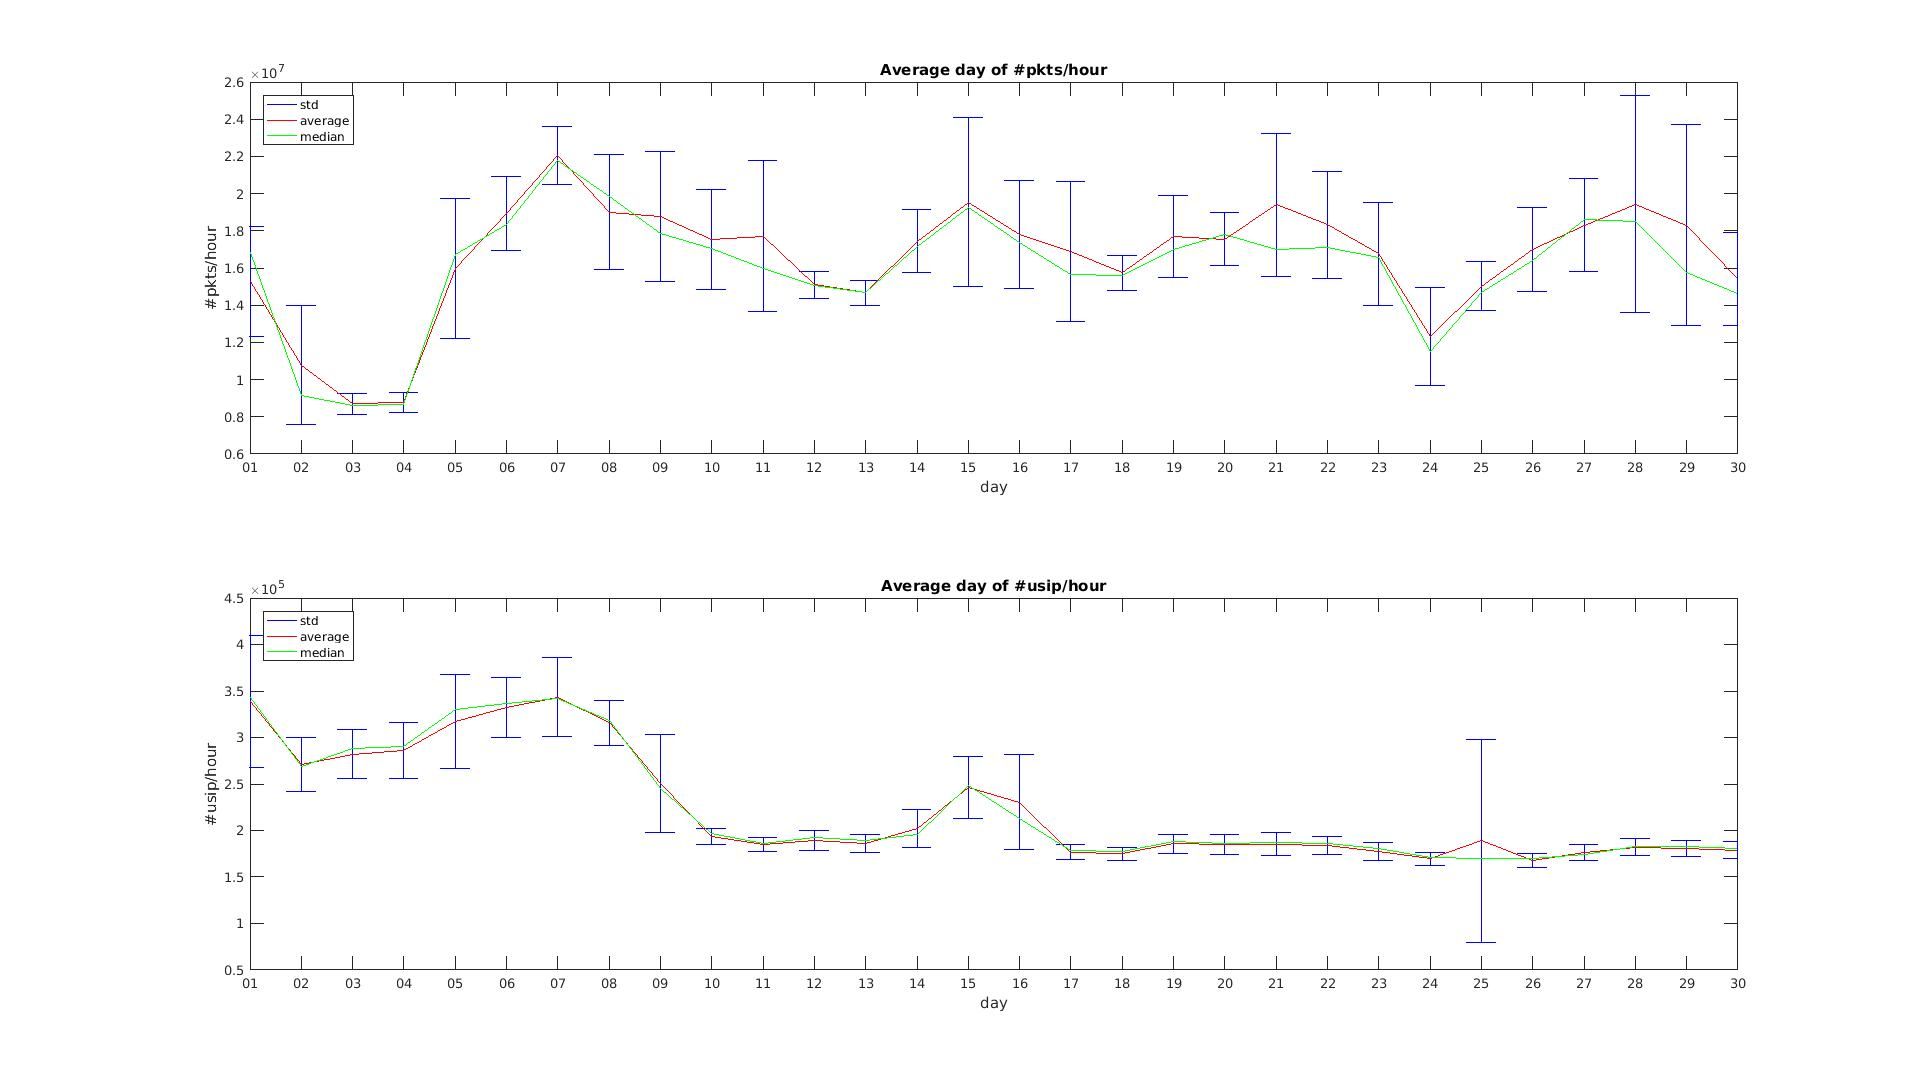
\includegraphics[width=1\textwidth]{./chapters/plots/rep-22.jpg}\\
\caption{ Average day of \#pkts/hour and \#usip/hour }
\end{figure}

\subsection*{rep-23}
\subsubsection*{a)}
The correlation factor between the mean \textit{\#pkts/hour} and mean \#usip/hour is $-0.062219840363756$. \\
The correlation factor between the median \textit{\#pkts/hour} and mean \#usip/hour is $0.053918525095147$.
\subsubsection*{b)}
As both coefficients are close to zero, there is no correlation between the mean and median  \textit{\#pkts/hour} and \textit{\#usip/hour} signals. 
\subsubsection*{c)}
The correlation was slightly higher when averaging the signal with 'mean', although we would have expected the 'median' to be higher. The reason for this assumption is, that the 'median' is more robust to outliers.
\subsubsection*{d)}
There is a peak on day 7 and 15 in both signals, but there are also peaks in the \textit{\#pkts/hour} signal, that do not appear in the \textit{\#usip/hour} signal on day 21 and 28. The peaks seem to appear weekly. This peaks could be caused by some botnet, that only operates in certain time intervals.